\subsection{PCP-Theorem}

\paragraph{Motivation}
Klasse NP auf PCP-Theorem aufbauen bzw. charakterisieren (anstatt mit Satz von Cook und SAT).
Reduktion von jedem Entscheidungsproblem in NP auf $GAP_{a,1}$(Max-SAT) für $a>1$.

\paragraph{Probabilistische Verifizierer}
Ein probabilistischer Verifizierer $V$ ist eine Polynomzeit-Turing-Maschine mit vier Bändern:
\begin{itemize}
    \item Eingabeband (endlich lang, lesen, Eingabe $x$)
    \item Arbeitsband (unendlich lang, lesen/schreiben), ``interner Arbeitsspeicher''
    \item Zufallsband (unendlich lang, lesen, Zufallsbits $\tau \in \binarystring$)
    \item Beweisband (endlich (aber sehr lang), Beweiskandidat $\pi \in \binarystring$ für $x \in L$)
\end{itemize}

Arbeitsweise:
\begin{enumerate}
    \item Lese $x$ und $\tau$ und berechne Indizes $i_1, ..., i_c$.
    \item Lese $\pi_{i_1}, ..., \pi_{i_c}$.
    \item Entscheide ob $x$ akzeptiert oder verworfen wird, abhängig von $\pi_{i_1}, ..., \pi_{i_c}, x, \tau$.
\end{enumerate}
$V$ schaut sich nur einen Teil des Beweiskandidats an!
Für ein fixes $\tau$ arbeitet $V$ deterministisch.
Verallgemeinerung von bekannten deterministischen Verifizierern, die kein Zufallsband haben.

Laufzeit: poly$(|x|)$ $\implies$ $c, |\tau| \in$ poly$(|x|)$ (aber $\pi$ unbeschränkt)

$V(x, \tau, \pi) \in$ \{accept, reject\}

\begin{figure}[h]
    \centering
    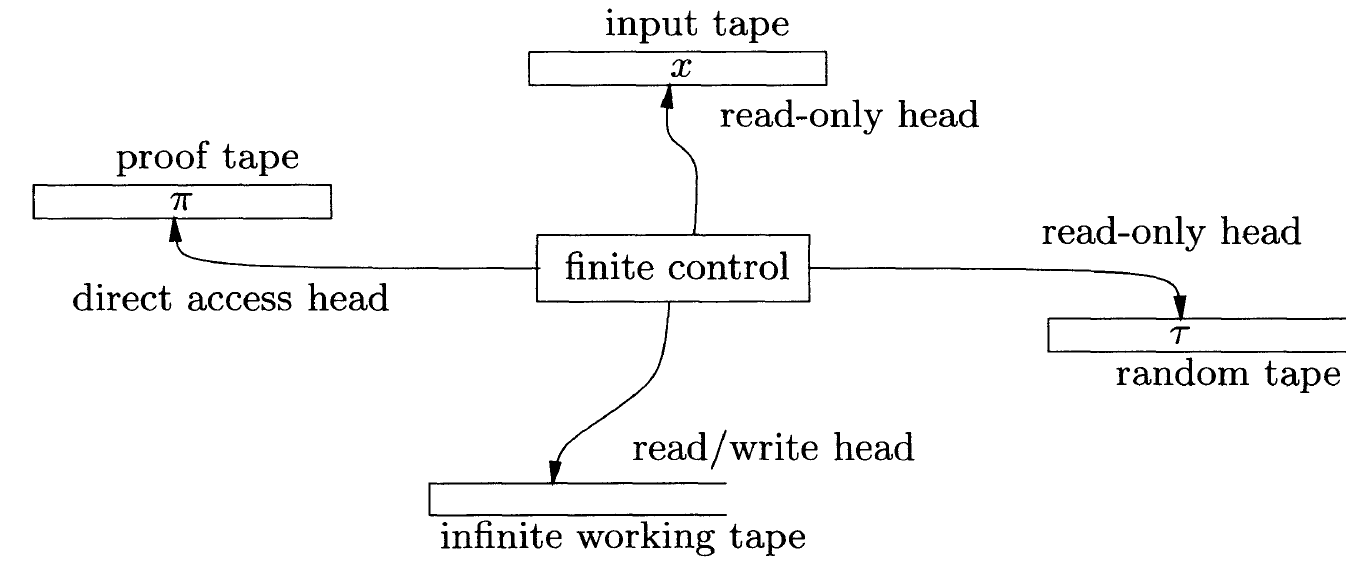
\includegraphics[width=0.6\textwidth]{images/prob-verifier.png}
    \caption{Probabilistischer Verifizierer als 4-Band-TM}
\end{figure}

\paragraph{Definition}
Seien $r, q \in \N \mapsto \N$.
Ein \emph{$(r(n), q(n))$-beschränkter probabilistischer Verifizierer} ist ein Verifizierer,
der für jede Eingabe $x$ nur $\leq r(n)$ Zufallsbits und $\leq q(n)$ Beweisbits liest, für $|x| = n$.

$V$ \emph{akzeptiert} Sprache $L$ falls gilt:
\begin{enumerate}[label=(\roman*)]
    \item Completeness: $ \forall x \in L \cl \exists \pi \; \forall \tau \cl V(x, \tau, \pi) = \text{accept} $
    \item Soundness: $ \forall x \notin L \cl \forall \pi \cl \Pr [ V(x, \tau, \pi) = \text{accept} ] \leq \frac{1}{2} $
\end{enumerate}
wobei $ \Pr [ V(x, \tau, \pi) = \text{accept} ] = \sum_{ \tau , V(x, \tau, \pi) = \text{accept} } \Pr [\tau] $.
\\
Annahme: Zufallsbits uniform verteilt, d.h. $\Pr [\tau] = \frac{1}{2^{|\tau|}}$.

\paragraph{Beispiel (SAT)}
$(0,n)$-beschränkter Verifizierer für SAT.
Liest $m \leq n = |\Phi|$ Beweisbits und interpretiert sie als Belegung für $x_1, ..., x_m$.
Akzeptiert $x$ wenn die Belegung $\Phi$ erfüllt. Deterministisch.

$\implies$ für alle Probleme in NP existiert ein deterministischer Polynomzeit-Verifizierer
(da SAT NP-vollständig ist).

\paragraph{Beispiel (GAP$_{1-\varepsilon, 1}$(E3SAT))}
für $\varepsilon \in (0,1)$.
Eingabe $\Phi$ ist entweder erfüllbar, oder ein Teil der $m$ Klauseln sind erfüllbar
(d.h. $ Opt_{Max-E3SAT}(\Phi) < (1-\varepsilon) \cdot m$).

Ziel:
$\left( \log_{1-\varepsilon}\frac{1}{2} \cdot \log n , 3 \cdot \log_{1-\varepsilon}\frac{1}{2} \right)$%
-beschränkter prob. Verifizierer.
Logarithmisch viele Zufallsbits, konstant viele Beweisbits.

Sei $\Phi = F_1 \wedge ... \wedge F_m$ eine E3-KNF-Formel über $x_1, ..., x_d$, $d \leq 3m$.
Sei $n = |\Phi| \geq 3m$, sei $k = \lceil \log_{1-\varepsilon}\frac{1}{2} \rceil$.
$V$ wählt zufällig $k$ Klausel-Indizes (= liest $k \cdot \lceil \log_2 m \rceil$ Zufallsbits).
$V$ interpretiert $\pi_1, ..., \pi_d$ als Belegung $\alpha$ für $x_1, ..., x_d$
(wobei es nur die $\leq 3k$ Belegungen der Variablen aus $F_{i1} \wedge ... \wedge F_{ik}$ lesen muss).
$V$ prüft ob $\alpha$ diese $k$ zufälligen Klauseln erfüllt.
Wenn ja akzeptiere, sonst verwerfe.

ad (i):
$\Phi$ erfüllbar $\implies \exists$ erfüllende Belegung/Beweis $\pi$ für die $V$ immer akzeptiert.

ad (ii):
$\Phi$ nicht erfüllbar $\implies$ $\forall$ Belegung erfüllt $< (1-\varepsilon) \cdot m$ Klauseln,
d.h. $\geq \varepsilon \cdot m$ sind nicht erfüllt.
\begin{align*}
    &\Pr [ \text{eine von $\alpha$ erfüllte Klausel zu wählen } ] \geq \frac{\varepsilon \cdot m}{m} = \varepsilon \\
\implies &\Pr [ \alpha \text{ erfüllt alle } F_{i1}, ..., F_{ik} ] \leq (1-\varepsilon)^k \\
\implies &\Pr [ V \text{ reject}]
    = \Pr [ \text{mind. eine Klausel von } F_{i1}, ..., F_{ik} \text{ nicht erfüllt} ] \\
    &\geq 1 - (1-\varepsilon)^k = 1 - (1-\varepsilon)^{ \lceil \log_{1-\varepsilon}\frac{1}{2} \rceil }
    \geq \frac{1}{2} \\
\implies &\Pr [ V \text{ accept} ] \leq \frac{1}{2}
\end{align*}

$\implies$ Mit Randomisierung können wir die Anzahl notwendiger/gelesener Beweisbits reduzieren,
selbst für schwere Probleme!
